\subsection{Election November 5, 2024: Biden vs Trump}
\begin{frame}[t]{Election November 5, 2024: Joe Biden}
\small

\begin{columns}[T, onlytextwidth]
\column{0.48\textwidth}
\vspace{-1em}
{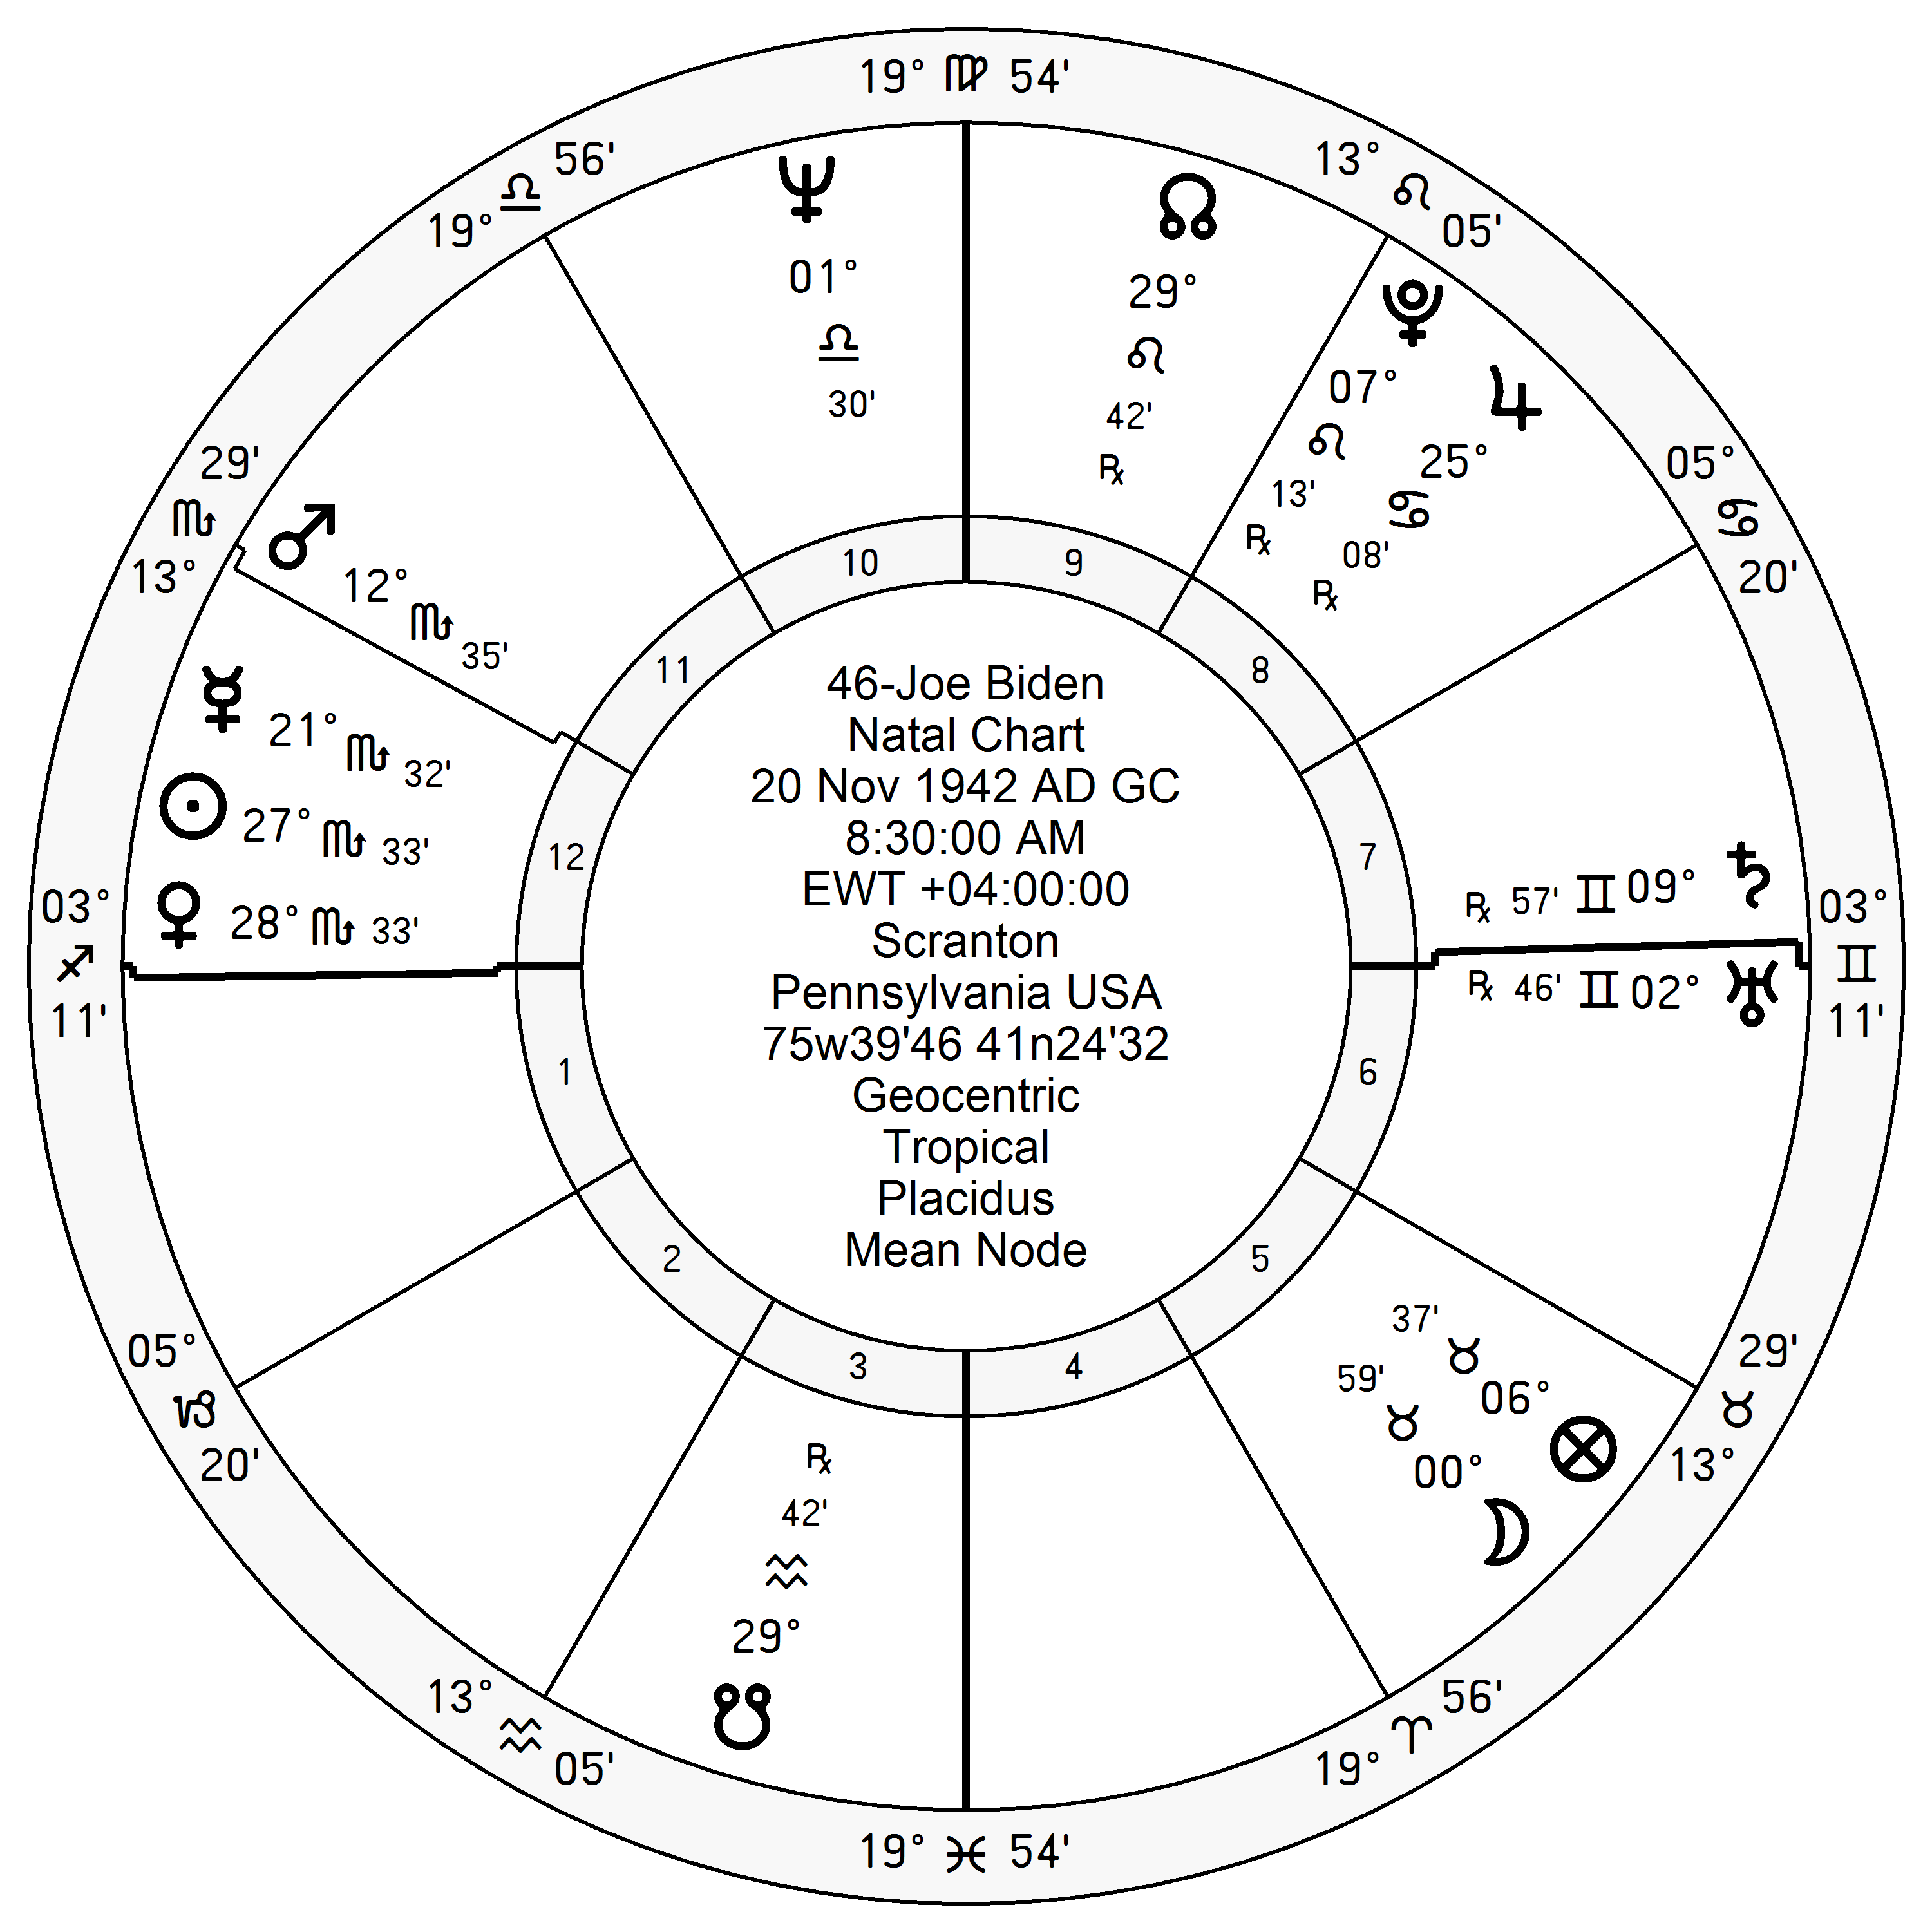
\includegraphics[width=0.9\textwidth]{charts/Biden.png}}
\fontsize{7pt}{8pt}\selectfont

\Mercury\, burnt \Sextile\, P1, \Sextile\, N10 \\
\Sun\, \Sextile\, P10; \Sextile\, N10

\column{0.48\textwidth}
\vspace{-1em}
{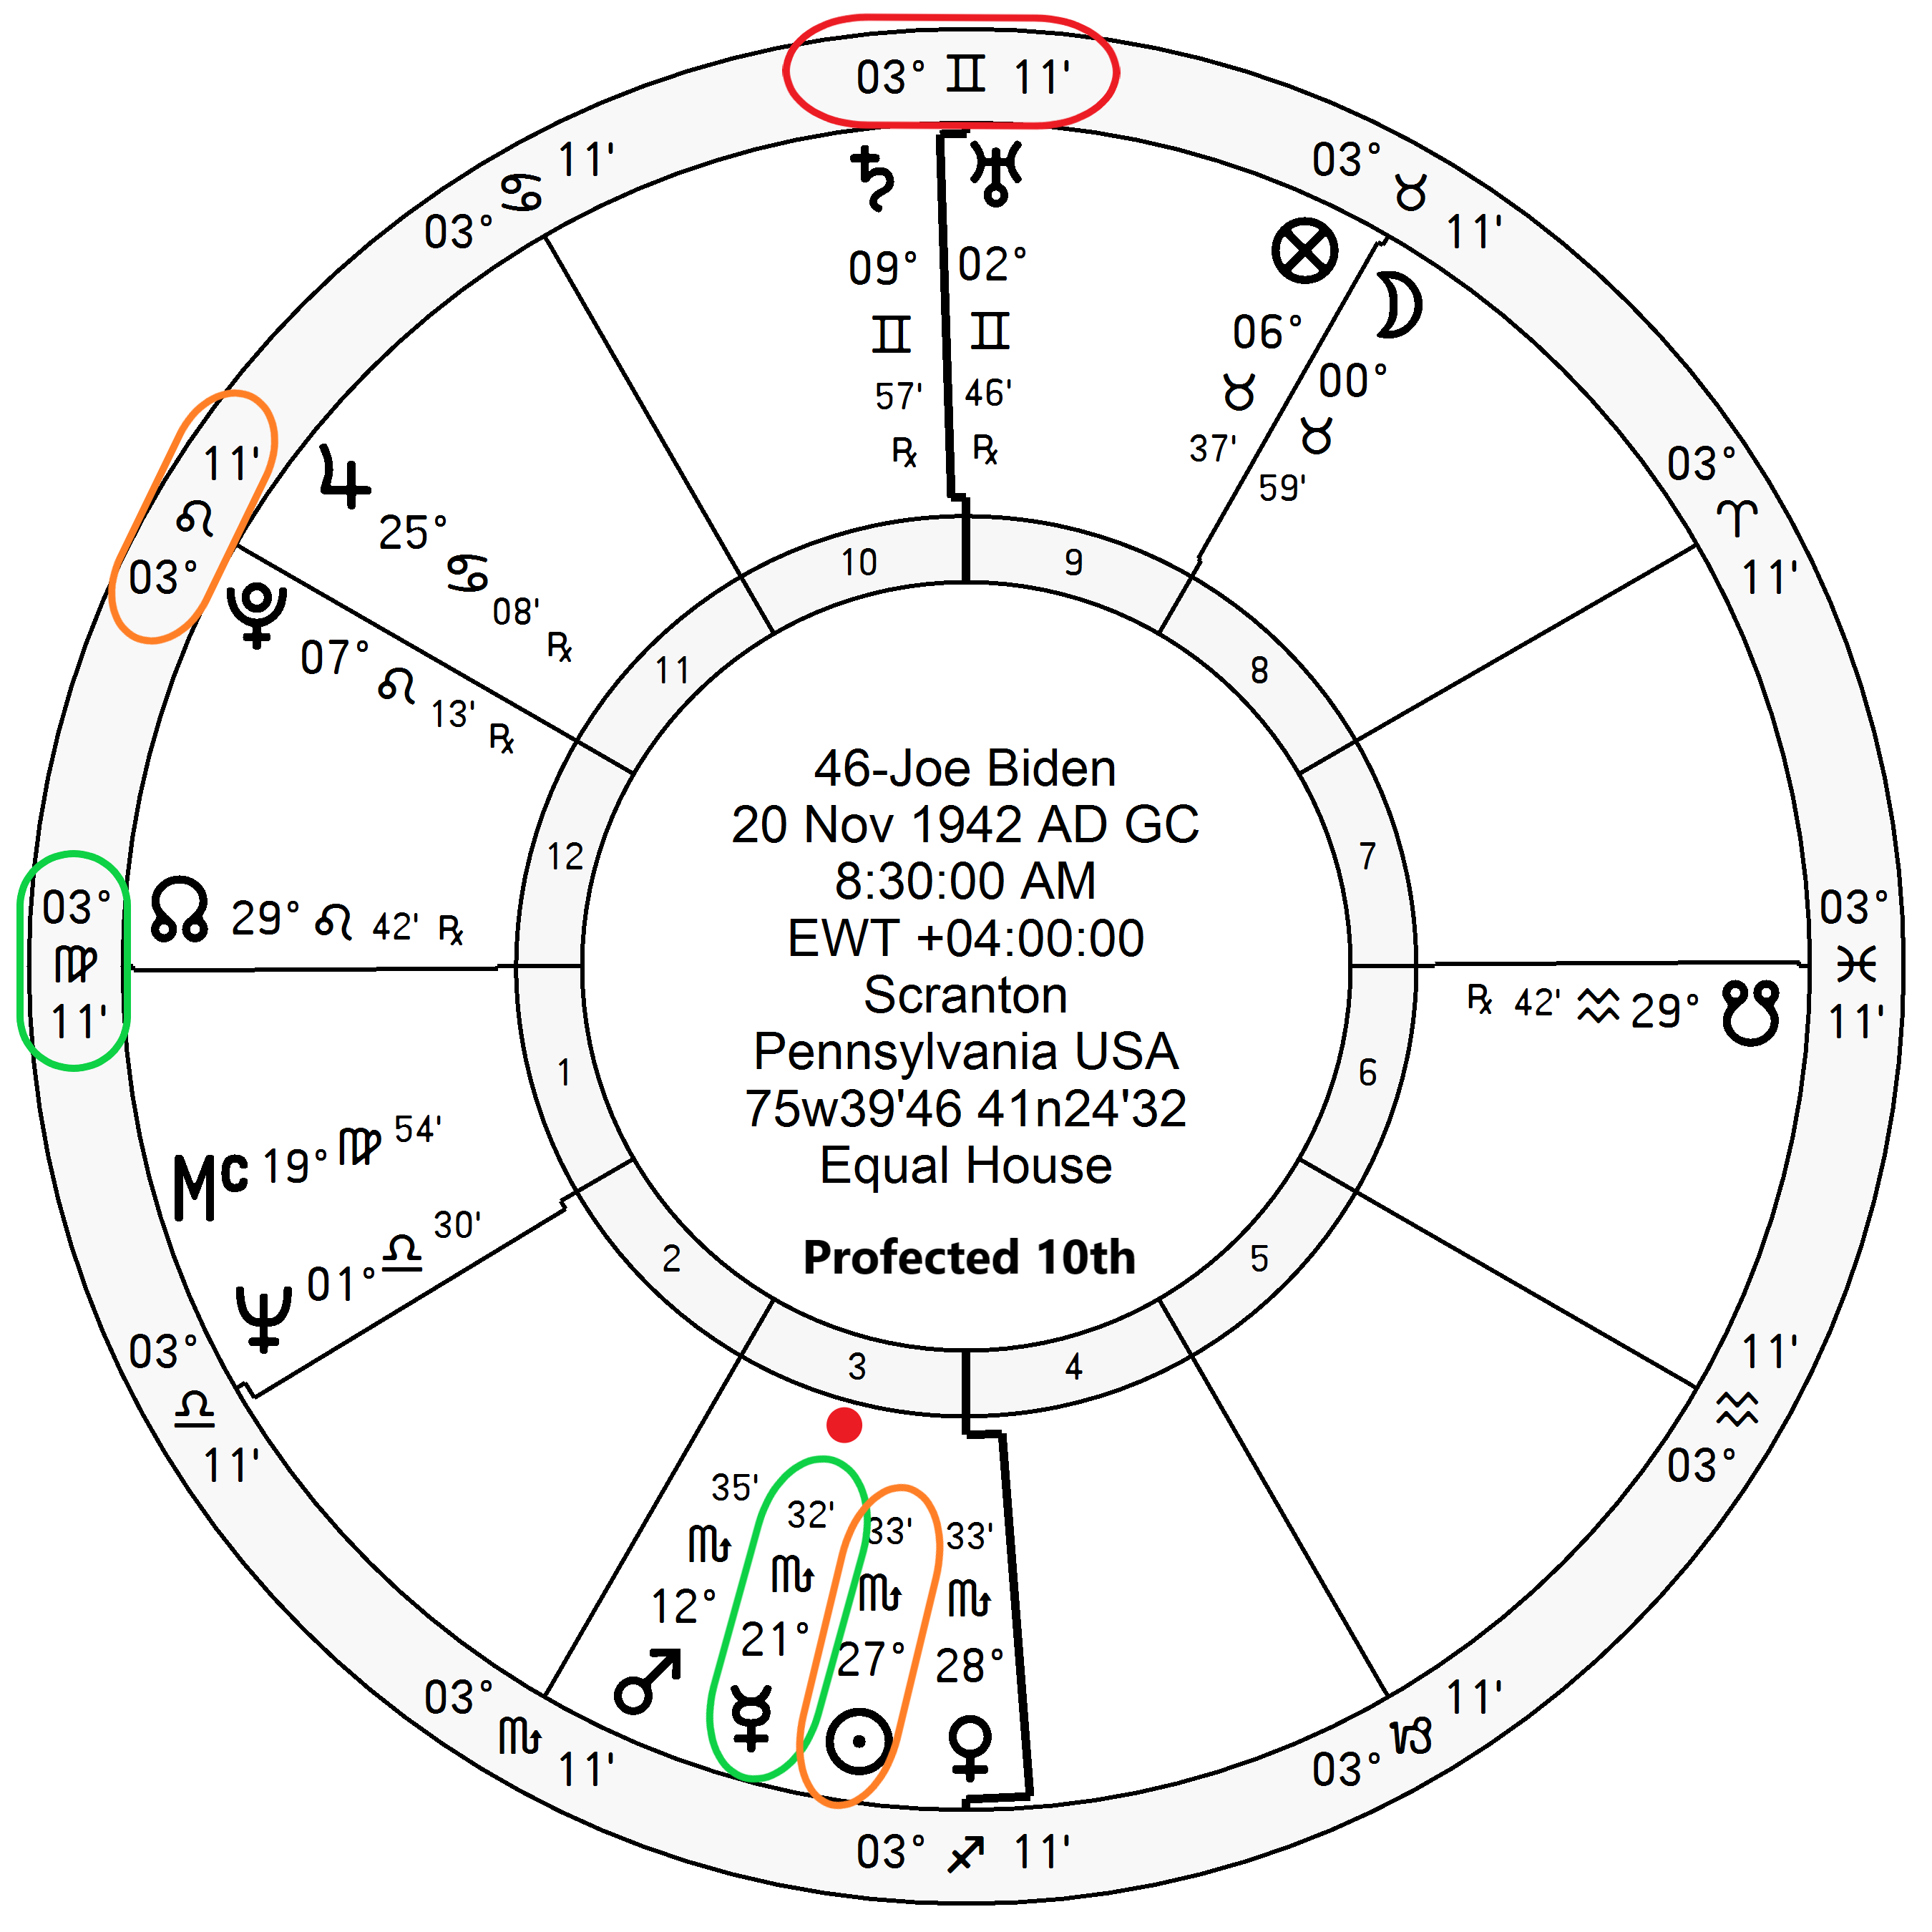
\includegraphics[width=0.9\textwidth]{charts/Biden-Prof-10th.png}}
\fontsize{8pt}{9pt}\selectfont

\textbf{\dgreen P1}=N10
	$\Rightarrow$ \Mercury\, (burnt) $\Rightarrow$ \textbf{\dgreen P3/N12}\\
\textbf{\red P10}=N7
	$\Rightarrow$ \Mercury\, (burnt) $\Rightarrow$ \textbf{\dgreen P3/N12}\\
PE=\textbf{\dgreen P12}/N9
	 $\Rightarrow$ \Sun\, $\Rightarrow$ \textbf{\dgreen P3/N12}

\end{columns}
\end{frame}

% ===================================================
\begin{frame}[t]{Election November 5, 2024: Donald Trump}
\small
\begin{columns}[T, onlytextwidth]
\column{0.48\textwidth}
\vspace{-1em}
{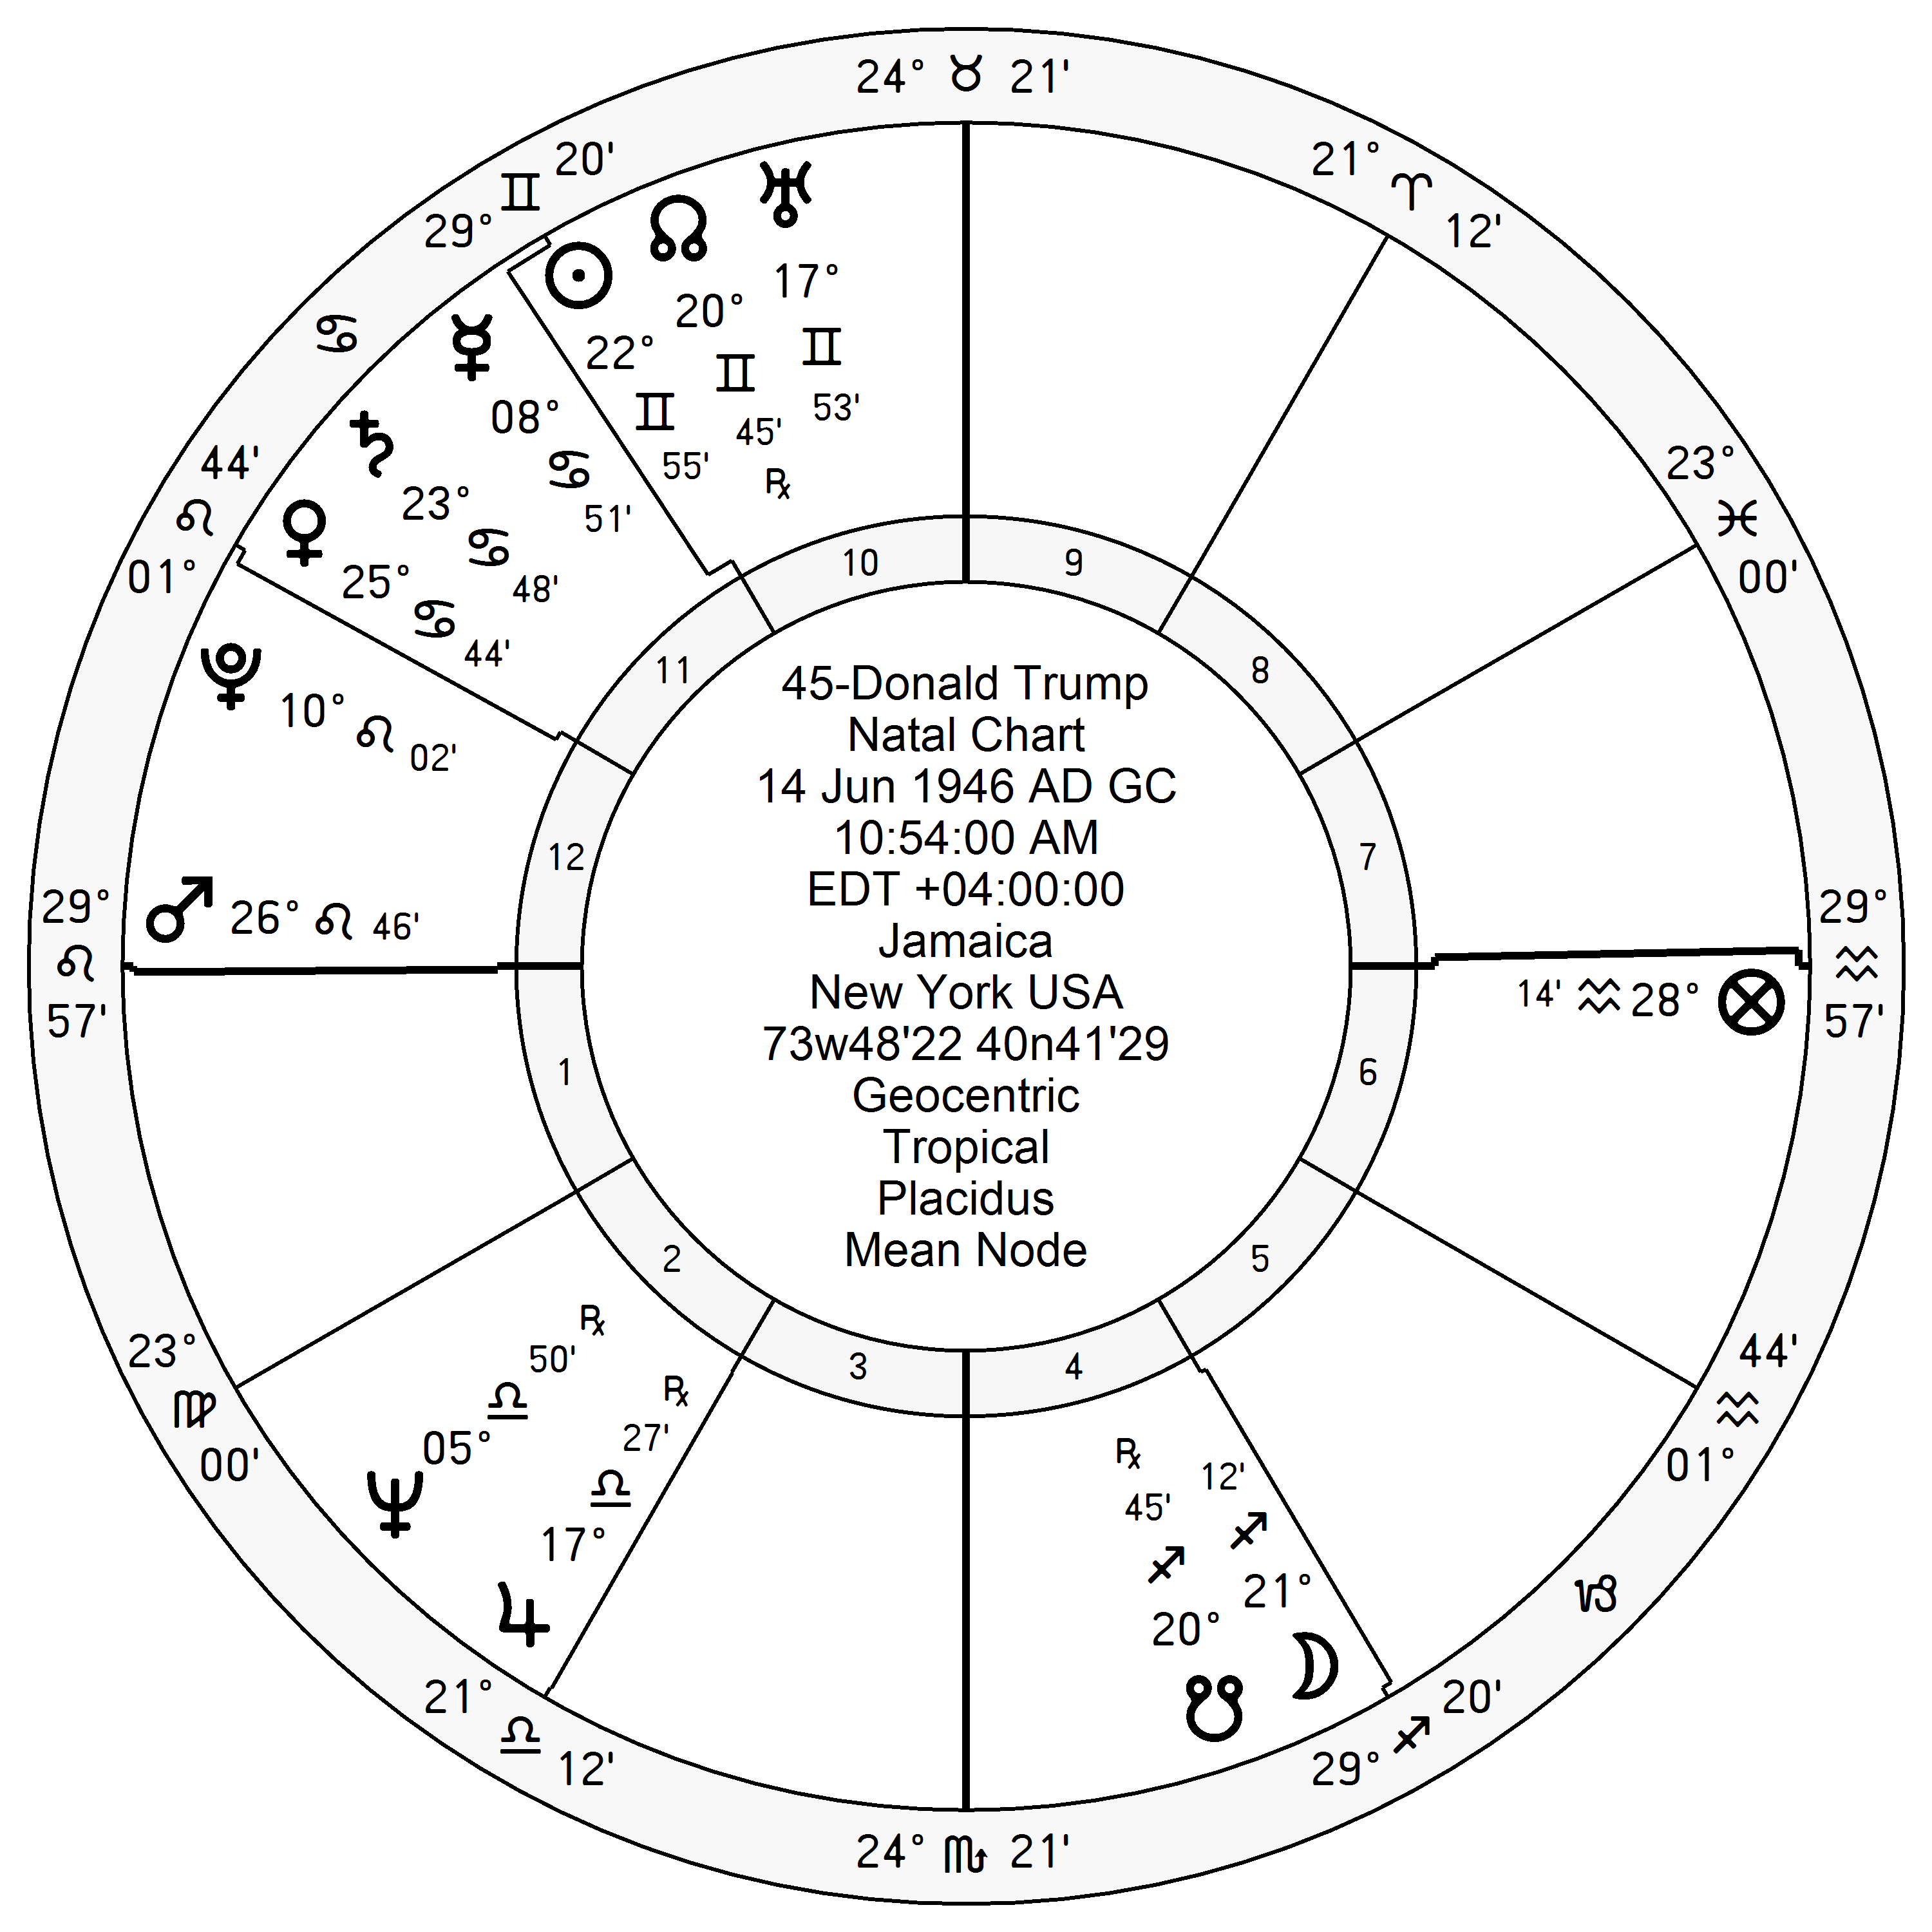
\includegraphics[width=0.9\textwidth]{charts/Trump.png}}
\fontsize{6pt}{7pt}\selectfont

\Saturn\, mit. \Quincunx\, (\Opposition) P10, \Trine\, P1, partile \Sextile\, to N2 \\
\Mars\, \Trine\, P10; \Square\, N10 \\
\Mercury\, \Trine\, P1, mit. \Quincunx\, (\Opposition) P10; \Sextile\, N1 \\
\vspace{0.5em}
Trump looks like the winner (assuming both are candidates on election day). The \SouthNode\, \Conjunction\, \Moon\, in P10 could cause problems, possibly GOP won't do well overall, weakening his control over Congress or the Senate, or both (\Moon\, rules P6, N11).

\column{0.48\textwidth}
\vspace{-1em}
{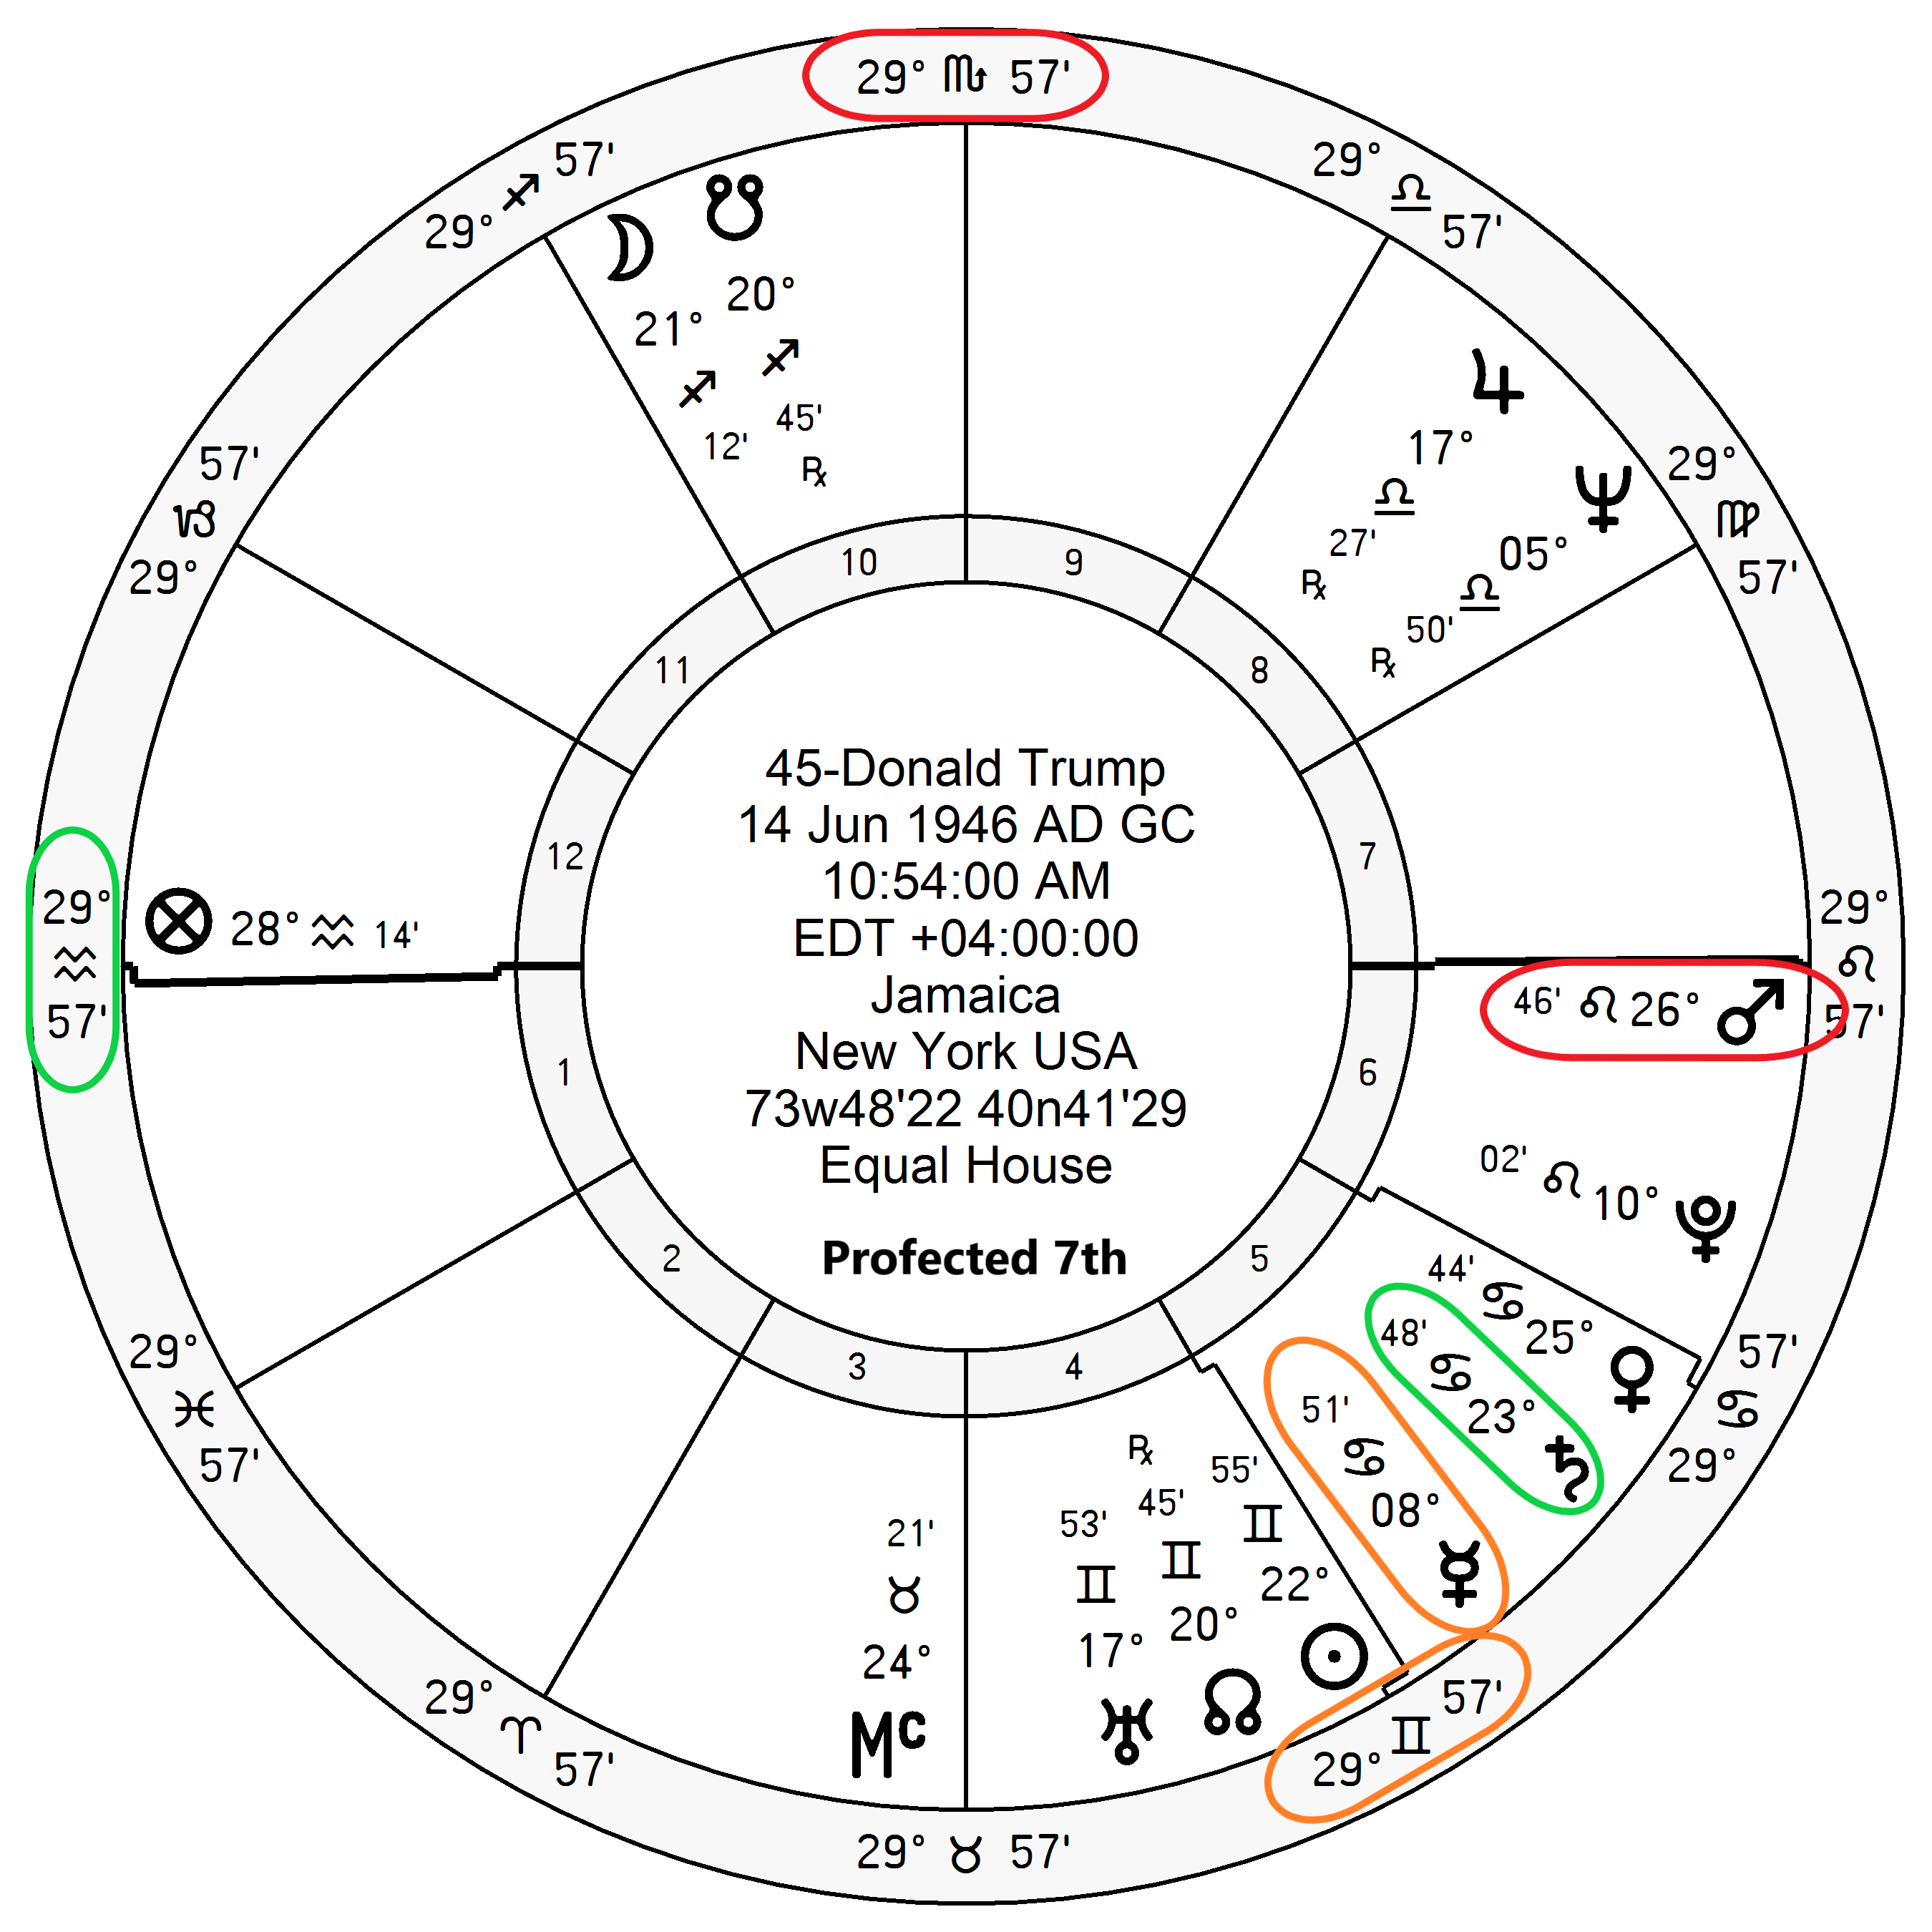
\includegraphics[width=0.9\textwidth]{charts/Trump-Prof-7th.png}}
\fontsize{8pt}{9pt}\selectfont
\textbf{\dgreen P1}=N7
	$\Rightarrow$ \Saturn\, $\Rightarrow$ \textbf{\dgreen P5/N11}\\
\textbf{\red P10}=N4
	$\Rightarrow$ \Mars\, $\Rightarrow$ P6/N12\\
PE=\textbf{\dgreen P5/N11}
	 $\Rightarrow$ \Mercury\, $\Rightarrow$ \textbf{\dgreen P5/N11}

\end{columns}
\end{frame}
